\documentclass[10pt,a4paper]{beamer}

\usepackage[utf8]{inputenc}
\usepackage[russian]{babel}
\usepackage[OT1]{fontenc}
\usepackage{amsmath}
\usepackage{amsfonts}
\usepackage{amssymb}
\usepackage{makeidx}
\usepackage{graphicx}
\usepackage{xcolor}
\usepackage{multirow}
\usepackage{framed}
\definecolor{shadecolor}{cmyk}{0,0,0,1}
\usepackage{hyperref}
\usepackage[normalem]{ulem}

\titlegraphic{
   
\includegraphics[width=4cm]{images/sfera.jpg}
}

\author{Николай Анохин \and Михаил Фирулик}
\title{Введение в Data Science \\ Занятие 8. Expectation Maximization}

\beamertemplatenavigationsymbolsempty

\begin{document}

\maketitle

\logo{
    
\includegraphics[width=4cm,keepaspectratio]{images/sfera.jpg}\hspace{0.45em}
}

\begin{frame}

\tableofcontents

\end{frame}

% ============================================== %

\section{K-Means и EM}

% ============================================== %

\begin{frame}{Задача кластеризации}

{\bf Дано} 
\begin{itemize}
\item обучающая выборка $\mathbf{X} = (\mathbf{x}_1, \ldots, \mathbf{x}_N)$
\item количество кластеров $K$
\end{itemize}

\vspace{1em}
{\bf Задача} \\
Разбить обучающую выборку на $K$ непересекающихся кластеров так, чтобы точки внутри одного кластера были близки, а точки из разных кластеров отдалены

\end{frame}

% ============================================== %

\begin{frame}{Критерий качества}

{\bf Пусть} 
\begin{itemize}
\item $\mu_k$ -- ``типичный'' представитель кластера $k$ (центроид)
\item $r_{nk}$ -- переменная принадлежности $\mathbf{x}_n$ к кластеру $C_k$
\[
r_{nk} = \begin{cases}
1, \text{ если } \mathbf{x}_n \in C_k \\
0, \text{ если } \mathbf{x}_n \not \in C_k \\
\end{cases}
\]
\end{itemize}

\vspace{1em}
Требуется выбрать $\mu_k$ и $r_{nk}$, которые {\bf минимизируют}
\[
J = \sum_{n=1}^N \sum_{k=1}^K r_{nk} \| \mathbf{x}_n - \mu_k \|^2
\]

\end{frame}

% ============================================== %

\begin{frame}{Оптимизация критерия}

\[
J = \sum_{n=1}^N \sum_{k=1}^K r_{nk} \| \mathbf{x}_n - \mu_k \|^2
\]

{\it Наблюдение:} оптимизировать одновременно и по $\mu_k$ и по $r_{nk}$ трудно \\
{\it Идея:} оптимизируем итеративно по очереди

\begin{itemize}
\item[E] При фиксированных $\mu_k$ подбираем оптимальные $r_{nk}$ \\
Члены с разными $n$ друг от друга не зависят, откуда
\[
r^*_{nk} = \begin{cases} 
1, \text{ если } k = \arg \min_j \| \mathbf{x}_n - \mu_j\|^2 \\
0, \text{ иначе }
\end{cases} 
\]
\item[M] При фиксированных $r_{nk}$ подбираем оптимальные $\mu_k$
\[
\mu_k = \frac{\sum_n r_{nk} \mathbf{x}_n}{\sum_n r_{nk}}
\]
\end{itemize}

\end{frame}

% ============================================== %

\begin{frame}{}

\begin{center}
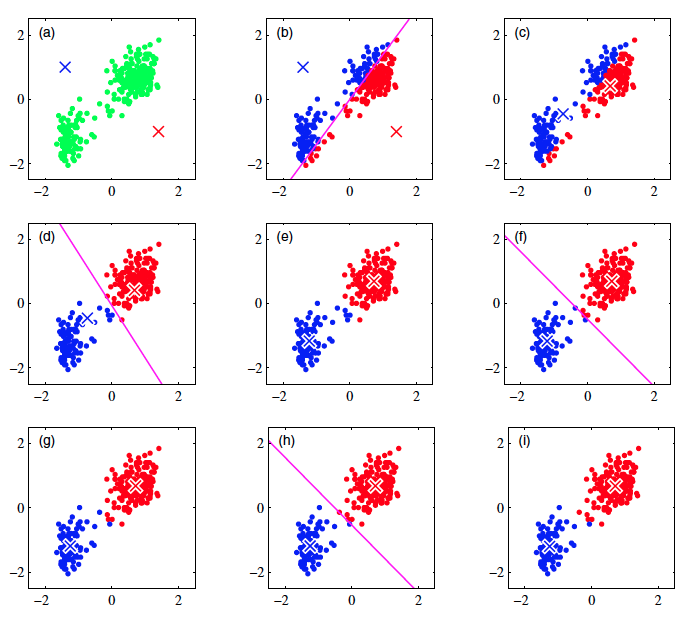
\includegraphics[scale=0.35]{images/kmeans.png}
\end{center}

\end{frame}

% ============================================== %

\begin{frame}{Алгоритм k-means}

\texttt{kmeans($\mathbf{X}$, $K$):}

\texttt{\quad Случайно задать $\mu_k$}

\texttt{\quad while(not converged):}

\texttt{\quad\quad for $n \in 1\ldots N$:}

\texttt{\quad\quad\quad $r^*_{nk} = int(k == \arg \min_j \| \mathbf{x}_n - \mu_j\|^2)$}

\texttt{\quad\quad for $k \in 1\ldots K$:}

\texttt{\quad\quad\quad $\mu_k = \frac{\sum_n r_{nk} \mathbf{x}_n}{\sum_n r_{nk}}$}

\texttt{\quad return $\mu_k$, $r_{nk}$}

\vspace{1em}
Алгоритмическая сложность: $O(NK)$

\end{frame}

% ============================================== %

\begin{frame}{Модификации}

\begin{itemize}
\item На каждом шаге работаем с $b$ случайно выбранными объектами из каждого кластера (mini-batch k-means) \\
\begin{center}
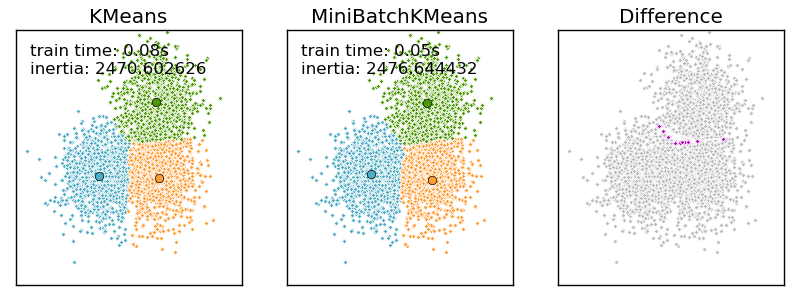
\includegraphics[scale=0.35]{images/mbatch.png}
\end{center}
\item Критерий качества (k-medoids)
\[
\tilde J = \sum_{n=1}^N \sum_{k=1}^K r_{nk} \nu(\mathbf{x}_n, \mu_k)
\]
$\mu_k$ -- один из объектов в кластере
\item Что если вхождение $\mathbf{x}$ в кластер $C_k$ описывается вероятностной функцией $p(\mathbf{x} | \theta_k)$? 
\end{itemize}

\end{frame}

% ============================================== %

\begin{frame}{Задача}

Кластеризовать объекты алгоритмом k-means

\begin{center}
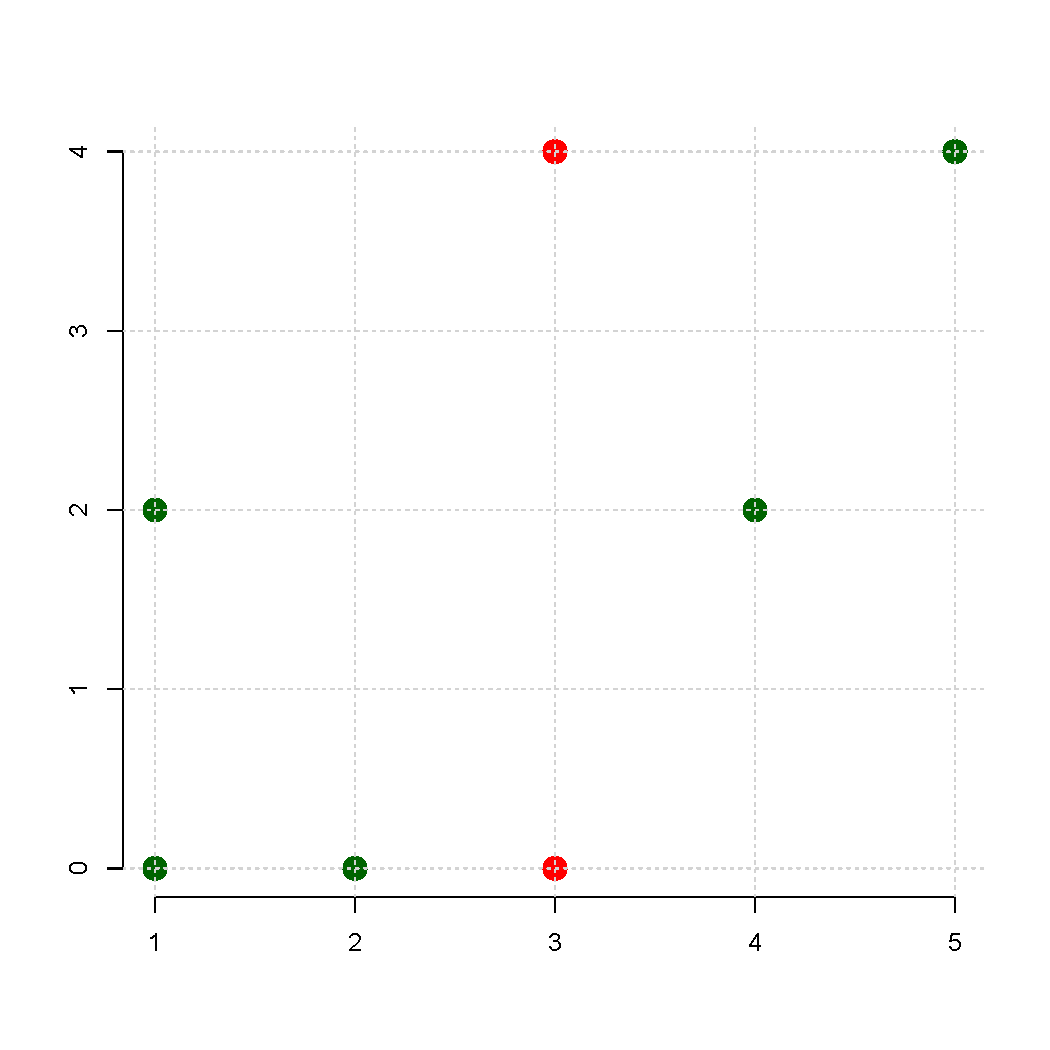
\includegraphics[scale=0.4]{images/problem.pdf}
\end{center}

\end{frame}

% ============================================== %

\begin{frame}{Многомерное гауссовское распределение}

Плотность вероятности
\[
\mathcal{N}(\mathbf{x} | \mu, \Sigma) = \frac{1}{(2\pi)^{D/2}}\frac{1}{|\Sigma|^{1/2}} \exp\left[{-\frac{1}{2} (\mathbf{x} - \mu)^T \Sigma^{-1} (\mathbf{x} - \mu)}\right]
\]
$\mu$ -- среднее, $\Sigma$ -- матрица ковариации

\begin{center}
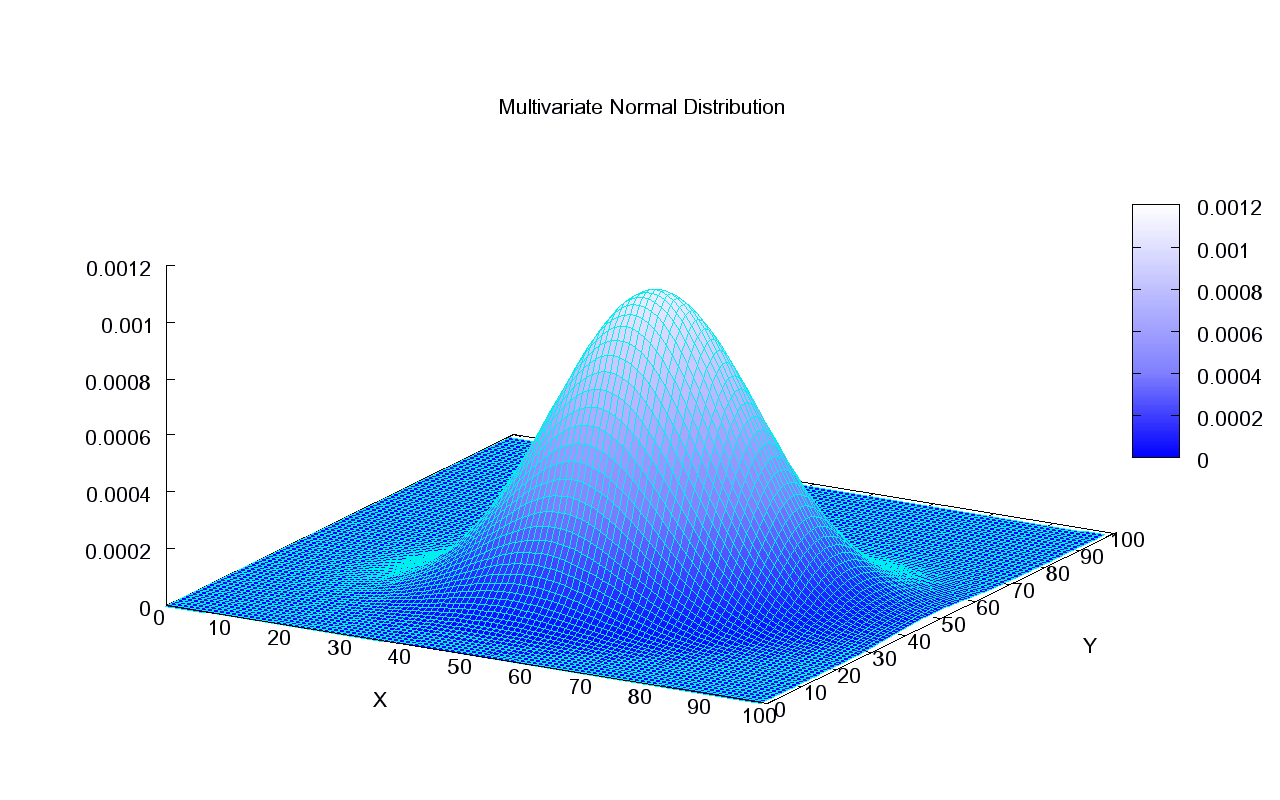
\includegraphics[scale=0.17]{images/multi.png}
\end{center}

\end{frame}

% ============================================== %

\begin{frame}{Смесь гауссовских распределений}

Введем скрытую переменную $\mathbf{z} = (z_1, \ldots, z_K)$ -- бинарный случайный вектор размерности $K$, такой что
\begin{enumerate}
\item $z_k \in \{0, 1\}$
\item $\sum_k z_k = 1$
\end{enumerate}
Тогда
\[
p(z_k = 1) = \pi_k, \;\; p(\mathbf{z}) = \prod_{k=1}^K \pi_k^{z_k}
\]
Гауссовское предположение
\[
p(\mathbf{x} | \mathbf{z}) = \mathcal{N} (\mathbf{x} | \mu_k, \Sigma_k), \;\; p(\mathbf{x}) = \sum_{k=1}^K \pi_k \mathcal{N} (\mathbf{x} | \mu_k, \Sigma_k)
\]

\end{frame}

% ============================================== %

\begin{frame}{}

``Ответственность'' $k$-го компонента за расположение объекта $x$
\[
\gamma(z_k) = p(z_k | \mathbf{x}) = \frac{\pi_k \mathcal{N} (\mathbf{x} | \mu_k, \Sigma_k)}{\sum_{j=1}^K \pi_j \mathcal{N} (\mathbf{x} | \mu_j, \Sigma_j)}
\]

\begin{center}
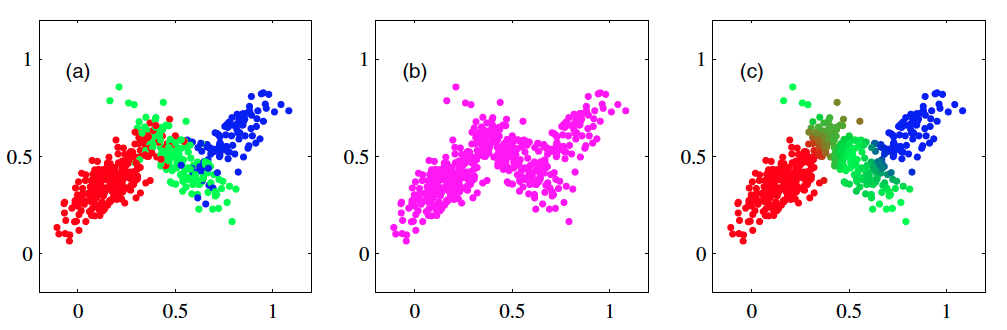
\includegraphics[scale=0.3]{images/gamma.png}
\end{center}

\end{frame}

% ============================================== %

\begin{frame}{Принцип максимального правдоподобия}

Log-likelihood
\[
\ln p(\mathbf{X} | \mathbf{\pi}, \mathbf{\mu}, \mathbf{\Sigma}) = \sum_{n=1}^N \ln \left[ \sum_{k=1}^K \pi_k \mathcal{N} (\mathbf{x}_n | \mu_k, \Sigma_k) \right]
\]
(Промежуточное) решение
\[
N_k = \sum_{n=1}^N \gamma(z_{nk}), \;\; \mu_k = \frac 1 {N_k} \sum_{n=1}^N \gamma(z_{nk}) \mathbf{x}_n
\]
\[
\Sigma_k = \frac 1 {N_k} \sum_{n=1}^N \gamma(z_{nk}) (\mathbf{x}_n - \mu_k)^T (\mathbf{x}_n - \mu_k)
\]
\[
\pi_k = \frac{N_k}{N}
\]

\end{frame}

% ============================================== %

\begin{frame}{EM-алгоритм: гауссовский случай}

\begin{enumerate}
\item[E] Expectation: при фиксированных $\mu_k, \Sigma_k, \pi_k$
\[
\gamma(z_{nk}) = \frac{\pi_k \mathcal{N} (\mathbf{x}_n | \mu_k, \Sigma_k)}{\sum_{j=1}^K \pi_j \mathcal{N} (\mathbf{x}_n | \mu_j, \Sigma_j)}
\]
\item[M] Maximization: при фиксированных $\gamma(z_{nk})$
\[
N_k = \sum_{n=1}^N \gamma(z_{nk}), \;\; \mu_k = \frac 1 {N_k} \sum_{n=1}^N \gamma(z_{nk}) \mathbf{x}_n
\]
\[
\Sigma_k = \frac 1 {N_k} \sum_{n=1}^N \gamma(z_{nk}) (\mathbf{x}_n - \mu_k)(\mathbf{x}_n - \mu_k)^T
\]
\[
\pi_k = \frac{N_k}{N}
\]
\item[S] Остановиться при достижении сходимости
\end{enumerate}

\end{frame}

% ============================================== %

\begin{frame}{}

\begin{center}
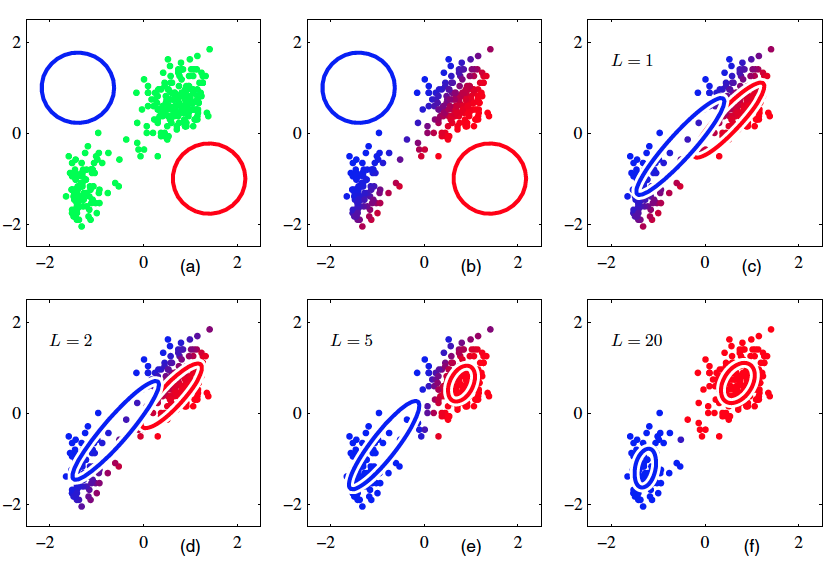
\includegraphics[scale=0.35]{images/gauss.png}
\end{center}

\end{frame}

% ============================================== %

\begin{frame}{EM-алгоритм: общий случай}

\begin{block}{Задача}
Пусть известно распределение $P(\mathbf{X}, \mathbf{Z} | \theta)$, где $\mathbf{x}$ -- наблюдаемые переменные, а $\mathbf{z}$ -- скрытые. Требуется найти $\theta$,  максимизирующее $P(\mathbf{X} | \theta)$.
\end{block}

\vspace{1em}
\begin{itemize}
\item[E] вычислить $P(\mathbf{Z} | \mathbf{X}, \theta^{old})$ при фиксированном $\theta^{old}$
\item[M] вычислить $\theta^{new} = \arg \max_{\theta} \mathcal{Q} (\theta, \theta^{old})$, где
\[
\mathcal{Q} (\theta, \theta^{old}) = E_\mathbf{Z}[\ln p(\mathbf{X}, \mathbf{Z} | \theta)] = \sum_{\mathbf{Z}} p(\mathbf{Z} | \mathbf{X}, \theta^{old}) \ln p(\mathbf{X}, \mathbf{Z} | \theta))
\]
\end{itemize}
{\it Улучшение:} ввести априорное распределение $p(\theta)$

\end{frame}

% ============================================== %

\begin{frame}{EM и K-means}

Пусть $\Sigma_k = \epsilon I$, тогда
\[
p(\mathbf{x} | \mu_k, \Sigma_k) = \frac{1}{\sqrt{2\pi\epsilon}}\exp(-\frac{1}{2\epsilon}\|\mathbf{x}-\mathbf{\mu_k}\|^2)
\]
\[
\gamma(z_{nk}) = \frac{\pi_k \exp(-\frac{1}{2\epsilon}\|\mathbf{x}-\mathbf{\mu_k}\|^2)}{\sum_j \pi_j \exp(-\frac{1}{2\epsilon}\|\mathbf{x}-\mathbf{\mu_j}\|^2)} \rightarrow r_{nk}
\]
\[
E_\mathbf{Z}[\ln p(\mathbf{X}, \mathbf{Z} | \mu, \Sigma, \pi)] \rightarrow -\sum_{n=1}^N \sum_{k=1}^K r_{nk} \| \mathbf{x}_n - \mu_k \|^2 + C
\]

\end{frame}

% ============================================== %

\begin{frame}{k-means: итог}

\begin{itemize}
\item[+] Скорость
\item[+] Простота
\item[--] Локальная сходимость
\item[--] Эллиптические кластеры
\end{itemize}

\end{frame}

% ============================================== %

\begin{frame}{Домашнее задание 1}

\begin{block}{k-means и модификации}
Реализовать алгоритм кластеризации k-means или одну из его модификаций (k-medoids, mini-batch) и протестировать на данных задачи модуля.
\end{block}

\vspace{1em}
Ключевые даты
\begin{itemize}
\item До 2014/04/26 00.00 выбрать ответственного
\item До 2014/05/03 00.00 предоставить решение (после -- половина очков)
\end{itemize}

\end{frame}

% ============================================== %

\section{Задача модуля}

% ============================================== %

\begin{frame}{Задача модуля}

\begin{tabular}{l p{5cm} p{3cm}}

\hline
\bf Источник & \bf Цель  & \bf Признаки \\
\hline
\raisebox{-0.8\height}{
\includegraphics[scale=0.12]{images/lastfm.jpg}}
& Кластеризовать музыкальных исполнителей так, чтобы в кластерах находились исполнители одного жанра 
& Текстовое описание, совместное участие в фестивалях \\
\hline
\raisebox{-0.8\height}{
\includegraphics[scale=0.12]{images/tomatoes.png}}
& Кластеризовать фильмы, так чтобы в кластерах находились фильмы одного жанра 
& Текстовое описание, общий актерский состав \\
\hline
\end{tabular}

\vspace{1em}
{\bf На выходе.} Построение и отбор признаков, реализация 2-3 алгоритмов кластеризации, визуализация кластеров, мини-отчет

\vspace{1em}
{\bf Выполнение.} Группы по 2-3 человека 

\vspace{1em}
{\bf Баллы.} 20 (индивидуально) + 10 (групповые -- поровну) 

\end{frame}

% ============================================== %

\begin{frame}{На сегодня}

\begin{enumerate}
\item Запускаем код из папки clustering
\item Делимся на группы
\item Выбираем, к какой задаче лежит душа
\begin{itemize}
\item Для LastFM \\
{\it Документация \url{http://www.lastfm.ru/api/intro}} \\
Задача: для каждого исполнителя загрузить список фестивалей
\item Для Rotten Tomatoes \\
{\it Документация \url{http://developer.rottentomatoes.com/docs}} \\
Задача: для каждого фильма загрузить список жанров
\end{itemize}
\item Думаем о \sout{добром} метриках расстояния
\end{enumerate}

\end{frame}

% ============================================== %

\end{document}